% =====================================================================
% BMED365 (Spring 2027) — Lab 4: Differentiable Neurosymbolic AI Report
% Printable Companion Notebook Export: 04_mechanistic_interpretability_and_biomarkers.ipynb
% Compile with: pdflatex 04_mechanistic_interpretability_and_biomarkers_ipynb.tex (run twice)
% =====================================================================
\documentclass[10pt,a4paper]{article}

\usepackage[utf8]{inputenc}
\usepackage[T1]{fontenc}
\usepackage[english]{babel}
\usepackage{lmodern}
\usepackage{microtype}
\usepackage{graphicx}
\usepackage{booktabs}
\usepackage{xltabular}
\usepackage{tabularx}
\usepackage{array}
\usepackage[table]{xcolor}
\usepackage{amsmath,amssymb,mathtools}
\usepackage{enumitem}
\usepackage[margin=1.7cm,top=1.75cm,bottom=1.85cm,headheight=14pt]{geometry}
\usepackage{fancyhdr}
\usepackage{lastpage}
\usepackage{titlesec}
\usepackage[most]{tcolorbox}
\usepackage{listings}
\usepackage{float}
\usepackage{caption}
\usepackage[hyphens]{url}
\usepackage[
    colorlinks=true,
    linkcolor=uibblue,
    citecolor=uibblue,
    urlcolor=uibred,
    bookmarksnumbered=true,
    bookmarksopen=true,
    pdftitle={04_mechanistic_interpretability_and_biomarkers.ipynb -- Mechanistic Interpretability and Whole-Organ Biomarkers (BMED365 Spring 2027)},
    pdfauthor={Arvid Lundervold (University of Bergen & MMIV) -- BMED365 Spring 2027},
    pdfsubject={BMED365 Spring 2027 -- Differentiable Neurosymbolic AI Companion Notebook}
]{hyperref}
\def\UrlBreaks{\do\/\do-\do_\do.}
% Allow clean line breaks after underscores in long filenames & Python identifiers
\let\origunderscore\_
\renewcommand{\_}{\origunderscore\allowbreak}

% =====================================================================
% COLORS (UiB / MMIV / BMED365 House Style)
% =====================================================================
\definecolor{uibblue}{RGB}{0, 61, 115}
\definecolor{uibred}{RGB}{175, 28, 44}
\definecolor{kiwigreen}{RGB}{27, 138, 90}
\definecolor{amberwarn}{RGB}{165, 95, 0}
\definecolor{amberbg}{RGB}{255, 250, 240}
\definecolor{lightgray}{RGB}{246, 248, 250}
\definecolor{rowalt}{RGB}{243, 247, 252}
\definecolor{codebg}{RGB}{245, 248, 252}
\definecolor{codehdr}{RGB}{224, 234, 246}
\definecolor{outbg}{RGB}{250, 250, 250}
\definecolor{outhdr}{RGB}{236, 238, 240}
\definecolor{codekw}{RGB}{0, 75, 145}
\definecolor{codestr}{RGB}{155, 35, 45}
\definecolor{codecmt}{RGB}{90, 105, 118}

% =====================================================================
% TYPOGRAPHY, HEADERS & CALLOUT BOXES
% =====================================================================
\setlength{\parindent}{0pt}
\setlength{\parskip}{0.42em}
\setlength{\emergencystretch}{1.8em}
\setlist[itemize]{topsep=2pt,itemsep=2pt,leftmargin=1.45em}
\setlist[enumerate]{topsep=2pt,itemsep=2pt,leftmargin=1.65em}

\newcolumntype{L}[1]{>{\raggedright\arraybackslash}p{#1}}
\newcolumntype{C}[1]{>{\centering\arraybackslash}p{#1}}
\newcolumntype{R}[1]{>{\raggedleft\arraybackslash}p{#1}}
\newcolumntype{Y}{>{\raggedright\arraybackslash}X}

\titleformat{\section}{\large\bfseries\color{uibblue}}{\thesection}{0.65em}{}[\vspace{1pt}\color{uibblue!40}\titlerule]
\titleformat{\subsection}{\normalsize\bfseries\color{uibblue!88!black}}{\thesubsection}{0.55em}{}
\titleformat{\subsubsection}{\small\bfseries\color{uibblue!75!black}}{\thesubsubsection}{0.5em}{}
\titlespacing*{\section}{0pt}{1.05em}{0.4em}
\titlespacing*{\subsection}{0pt}{0.75em}{0.25em}
\titlespacing*{\subsubsection}{0pt}{0.55em}{0.2em}

\pagestyle{fancy}
\fancyhf{}
\fancyhead[L]{\footnotesize\textcolor{gray}{BMED365 (Spring 2027) $\cdot$ Neurosymbolic 7\,T MRI Package}}
\fancyhead[R]{\footnotesize\textcolor{gray}{\texttt{04\_mechanistic\_interpretability\_and\_biomarkers.ipynb}}}
\fancyfoot[L]{\footnotesize\textcolor{gray}{University of Bergen \& MMIV $\cdot$ \href{https://github.com/arvidl/BMED365-2027}{\textcolor{gray}{github.com/arvidl/BMED365-2027}}}}
\fancyfoot[R]{\footnotesize\textcolor{gray}{Page \thepage{} of \pageref{LastPage}}}
\renewcommand{\headrulewidth}{0.4pt}
\renewcommand{\footrulewidth}{0.2pt}

\fancypagestyle{firstpage}{
    \fancyhf{}
    \fancyfoot[L]{\footnotesize\textcolor{gray}{University of Bergen \& MMIV $\cdot$ \href{https://github.com/arvidl/BMED365-2027}{\textcolor{gray}{github.com/arvidl/BMED365-2027}}}}
    \fancyfoot[R]{\footnotesize\textcolor{gray}{Page \thepage{} of \pageref{LastPage}}}
    \renewcommand{\headrulewidth}{0pt}
    \renewcommand{\footrulewidth}{0.2pt}
}

% --- Notebook Cell & Pedagogical Boxes ---
\newtcolorbox{seqbox}[1][]{
    enhanced, breakable,
    colback=lightgray, colframe=uibblue,
    colbacktitle=uibblue, coltitle=white,
    fonttitle=\bfseries\small, title={#1},
    boxrule=0.6pt, arc=2.5pt, left=7pt, right=7pt, top=5pt, bottom=5pt
}

\newtcolorbox{codebox}[1][]{
    enhanced, breakable,
    colback=codebg, colframe=uibblue!35,
    colbacktitle=codehdr, coltitle=uibblue!90!black,
    fonttitle=\ttfamily\scriptsize\bfseries, title={#1},
    boxrule=0.55pt, arc=2.2pt, left=6pt, right=6pt, top=3pt, bottom=3pt,
    toptitle=2.5pt, bottomtitle=2.5pt
}

\newtcolorbox{outbox}[1][]{
    enhanced, breakable,
    colback=outbg, colframe=gray!45,
    colbacktitle=outhdr, coltitle=black!75,
    fonttitle=\ttfamily\scriptsize\bfseries, title={#1},
    boxrule=0.5pt, arc=2.2pt, left=6pt, right=6pt, top=3pt, bottom=3pt,
    toptitle=2pt, bottomtitle=2pt
}

\newtcolorbox{clinbox}[1][]{
    enhanced, breakable,
    colback=amberbg, colframe=amberwarn,
    colbacktitle=amberwarn, coltitle=white,
    fonttitle=\bfseries\small, title={#1},
    boxrule=0.6pt, arc=2.5pt, left=7pt, right=7pt, top=5pt, bottom=5pt
}

\newtcolorbox{guidehdr}[1][]{
    enhanced,
    colback=kiwigreen!6, colframe=kiwigreen!75!black,
    borderline west={2.5pt}{0pt}{kiwigreen!85!black},
    boxrule=0.45pt, arc=2pt, left=7pt, right=7pt, top=3.5pt, bottom=3.5pt,
    before skip=0.7em, after skip=0.35em
}

% --- Listings Styles (UTF-8 literate support for pdflatex) ---
\lstdefinestyle{pybmed}{
    language=Python,
    basicstyle=\ttfamily\scriptsize,
    keywordstyle=\bfseries\color{codekw},
    stringstyle=\color{codestr},
    commentstyle=\itshape\color{codecmt},
    showstringspaces=false,
    breaklines=true,
    breakatwhitespace=false,
    breakindent=12pt,
    columns=fullflexible,
    keepspaces=true,
    upquote=true,
    aboveskip=2pt,
    belowskip=2pt,
    xleftmargin=0pt,
    xrightmargin=0pt,
    literate={±}{{$\pm$}}1
             {³}{{\textsuperscript{3}}}1
             {×}{{$\times$}}1
             {é}{{\'e}}1
             {ö}{{\"o}}1
             {Ł}{{\L{}}}1
             {Δ}{{$\Delta$}}1
             {α}{{$\alpha$}}1
             {–}{{--}}1
             {—}{{---}}1
             {≥}{{$\ge$}}1
             {≤}{{$\le$}}1
             {⊂}{{$\subset$}}1
             {∈}{{$\in$}}1
             {→}{{$\to$}}1
             {…}{{\ldots}}1
}

\lstdefinestyle{bashbmed}{
    language=bash,
    basicstyle=\ttfamily\scriptsize,
    keywordstyle=\bfseries\color{codekw},
    stringstyle=\color{codestr},
    commentstyle=\itshape\color{codecmt},
    showstringspaces=false,
    breaklines=true,
    breakatwhitespace=false,
    breakindent=12pt,
    columns=fullflexible,
    keepspaces=true,
    upquote=true,
    aboveskip=2pt,
    belowskip=2pt,
    xleftmargin=0pt,
    xrightmargin=0pt
}

\lstdefinestyle{outbmed}{
    basicstyle=\ttfamily\scriptsize\color{black!85},
    showstringspaces=false,
    breaklines=true,
    breakatwhitespace=false,
    columns=fullflexible,
    keepspaces=true,
    upquote=true,
    aboveskip=1pt,
    belowskip=1pt,
    xleftmargin=0pt,
    xrightmargin=0pt
}

\lstdefinestyle{outbmedwide}{
    basicstyle=\ttfamily\fontsize{6.3pt}{7.6pt}\selectfont\color{black!85},
    showstringspaces=false,
    breaklines=true,
    breakatwhitespace=false,
    columns=fullflexible,
    keepspaces=true,
    upquote=true,
    aboveskip=1pt,
    belowskip=1pt,
    xleftmargin=0pt,
    xrightmargin=0pt
}

\newcommand{\ghblob}{https://github.com/arvidl/BMED365-2027/blob/main}
\newcommand{\colabbase}{https://colab.research.google.com/github/arvidl/BMED365-2027/blob/main}
\newcommand{\repodir}{Lab4-Comp-Imag/Kiwi-challenge/docs/neurosymbolic-report}
\newcommand{\colabbtn}[1]{%
  \href{#1}{\tcbox[on line, arc=2.5pt, boxsep=0pt, left=6pt, right=6pt, top=2.5pt, bottom=2.5pt,
    colback=amberwarn!85!yellow, colframe=white!70!amberwarn, boxrule=0.5pt]{%
    \sffamily\bfseries\scriptsize\color{white}Open in Google Colab}}%
}

% =====================================================================
\begin{document}
\thispagestyle{firstpage}

% --- TITLE BANNER ---
\begin{tcolorbox}[
    enhanced, colback=uibblue, colframe=uibblue,
    arc=3.5pt, left=12pt, right=12pt, top=9pt, bottom=9pt
]
{\Large\bfseries\color{white} Companion Notebook 04 --- Mechanistic Interpretability, Division of Labor \& Whole-Organ Biomarkers\\[2pt]
{\large Causal $z_{\text{GPS}}$ Inspection, Mat\'ern Hard-Core Split Sensitivity, Error Anatomy \& 128-Slice NIfTI Export}}\\[4pt]
{\normalsize\color{white!90} BMED365 --- Computational Imaging, Modeling and AI in Biomedicine (Spring 2027)}\\[3pt]
{\footnotesize\color{white!84}
Arvid Lundervold (University of Bergen \& MMIV) $\;\cdot\;$ Reproduces Report Sec.\ 3.4, Figs.\ 8--9 \& Tables~7--8 $\;\cdot\;$ Measured runtime: \texttt{99.3 s} (MPS)
}\\[6pt]
\colabbtn{\colabbase/\repodir/notebooks/04_mechanistic_interpretability_and_biomarkers.ipynb}\hspace{8pt}
{\footnotesize\href{\ghblob/\repodir/notebooks/04_mechanistic_interpretability_and_biomarkers.ipynb}{\textcolor{white}{\underline{\texttt{04\_mechanistic\_interpretability\_and\_biomarkers.ipynb} on GitHub}}}}\hspace{10pt}
{\footnotesize\href{\ghblob/\repodir/neurosymbolic-kiwi-report.pdf}{\textcolor{white}{\underline{Technical Report PDF}}}}
\end{tcolorbox}

\begin{seqbox}[Neurosymbolic 7\,T MRI Technical Report --- Companion Package (\texttt{docs/neurosymbolic-report})]
{\footnotesize Companion to \href{\ghblob/\repodir/neurosymbolic-kiwi-report.pdf}{\textbf{\texttt{neurosymbolic-kiwi-report.pdf}}} and shared library \href{\ghblob/\repodir/notebooks/kiwi_ns_lib.py}{\texttt{kiwi\_ns\_lib.py}} (\href{\ghblob/\repodir/notebooks/kiwi_ns_lib_py.pdf}{\textit{annotated PDF}}):}
\begin{enumerate}[start=1, itemsep=1.2pt, topsep=2pt, font=\footnotesize]
    \item \href{\ghblob/\repodir/notebooks/01_data_geometry_and_prior_audit.ipynb}{\texttt{01\_data\_geometry\_and\_prior\_audit.ipynb}} --- 7\,T MRI geometry, empirical audit of Priors 1--3, tri-planar Micro-GT superimposition \& manual GT editing guide (Figs.\ 1--3, Table~3; 27.4\,s MPS).
    \item \href{\ghblob/\repodir/notebooks/02_instancenorm_trap_and_ltn_math.ipynb}{\texttt{02\_instancenorm\_trap\_and\_ltn\_math.ipynb}} --- Experimental proof of \texttt{InstanceNorm3d} coordinate erasure, Bayes Log-Odds \texttt{Organ-GPS}, fuzzy $T$-norms \& LTN $p$-mean autograd sweep (Figs.\ 4--5, Table~4; 7.2\,s MPS).
    \item \href{\ghblob/\repodir/notebooks/03_multiseed_ablation_and_calibration.ipynb}{\texttt{03\_multiseed\_ablation\_and\_calibration.ipynb}} --- 3-seed $\times$ 6-model controlled ablation, operating-point calibration shift \& unmasked whole-organ OOD safety (Figs.\ 6--7, Tables~5--6; 555.1\,s MPS).
    \item \textbf{\texttt{04\_mechanistic\_interpretability\_and\_biomarkers.ipynb} (this notebook)} --- Causal neural--symbolic division of labor ($z_{\text{GPS}}$), Mat\'ern hard-core split sweep, error anatomy \& 128-slice NIfTI biomarkers (Figs.\ 8--9, Tables~7--8; 99.3\,s MPS).
    \item \href{\ghblob/\repodir/notebooks/05_axiom_stress_tests_and_clinical_translation.ipynb}{\texttt{05\_axiom\_stress\_tests\_and\_clinical\_translation.ipynb}} --- Pathological mass-effect center-shift ($\Delta r \in [0, 8]$\,mm) \& radial-scale ($\alpha \in [0.80, 1.25]$) stress tests vs.\ rigid post-hoc masks (Fig.\ 10, Table~9; 55.4\,s MPS).
\end{enumerate}
\end{seqbox}

\subsection*{Purpose}
Because \texttt{AdditiveBayesOrganNet3D} decomposes seed log-odds explicitly as $z_{\text{total}} = z_{\text{app}}(\mathbf{X}) + z_{\text{GPS}}(r/R, |2z/Z - 1|)$, we can open the learned brain and prove \textbf{four mechanistic discoveries}:
\begin{enumerate}
\item \textbf{Causal Neural--Symbolic Division of Labor:} Train the exact same \texttt{AdditiveBayesOrganNet3D} \textbf{with} vs. \textbf{without} central-columella hard-negatives (\texttt{X\_ng}), proving causally that \texttt{Organ-GPS} automatically erects an inner columella barrier at $r/R < 0.22$ when \texttt{z\_app} has no columella supervision, and delegates the columella to \texttt{z\_app} when \texttt{X\_ng} is present!
\item \textbf{Zoomed Declarative \texttt{Lab 5} Hard-Core Clump Split \& Cutoff Sensitivity:} Inspect an actual split twin-seed clump and sweep \texttt{split\_mm3 $\in$ [2.2, 3.0]}.
\item \textbf{Physical Error Anatomy (\texttt{TP} vs. \texttt{FN}):} Quantify volume, $T_2$ contrast drop, and $z$-border proximity of missed seeds.
\item \textbf{Whole-Fruit 128-Slice Unmasked Biomarkers:} Compute $V_{\text{kiwi}}$, raw \& Micro-GT calibrated seed counts, median seed volume, and ``lesion load'' $V_{\text{seeds}} / V_{\text{kiwi}}$.
\end{enumerate}

\section*{0. Environment Setup: Portable Execution, Shared Models \& NIfTI Export Pipeline}
\addcontentsline{toc}{section}{\texorpdfstring{0. Environment Setup: Portable Execution, Shared Models \& NIfTI Export Pipeline}{0. Environment Setup: Portable Execution, Shared Models and NIfTI Export Pipeline}}

\begin{guidehdr}
{\small\bfseries\color{kiwigreen!75!black}Conceptual \& Practical Motivation}
\end{guidehdr}
Before opening the learned Bayesian spatial log-prior and extracting whole-organ quantitative biomarkers, this setup cell configures a reproducible local/\allowbreak{}Colab runtime:

\begin{itemize}
\item \textbf{Zero-drift shared library (\texttt{kiwi\_ns\_lib.py}):} Loads the exact \texttt{AdditiveBayesOrganNet3D} architecture, training routine, hard-core clump splitter, Hungarian instance matcher (\texttt{match\_instance\_sets}), and bit-aligned NIfTI writer (\texttt{save\_aligned\_label\_nifti}) shared across all five companion notebooks.
\item \textbf{Scientific \& 3D imaging stack:} \texttt{torch} runs 100-epoch training and noiseless \texttt{gps\_log\_prior} forward sweeps; \texttt{scipy.spatial.distance.cdist} and \texttt{skimage.measure.regionprops} measure physical 3D sub-centroid spacings and error-anatomy statistics; \texttt{nibabel} exports our final whole-fruit 3D instance mask (\texttt{kiwi\_neurosymbolic\_pred\_labels.nii.gz}) bit-aligned to the original 7\,T MRI.
\item \textbf{Runtime device \& paths:} \texttt{kns.get\_best\_device()} selects \texttt{CUDA} $\to$ Apple \texttt{MPS} $\to$ \texttt{CPU}, and \texttt{kns.resolve\_report\_dirs()} locates \texttt{FIG\_DIR} and \texttt{RES\_DIR} for Figures 7--8 and \texttt{nb04\_mechanistic\_and\_whole\_organ.json}.
\end{itemize}

\begin{codebox}[{In [1] $\cdot$ Python --- Environment setup, shared models \& bit-aligned NIfTI export pipeline}]
\begin{lstlisting}[style=pybmed]
import json
import sys
import urllib.request
from pathlib import Path

# Auto-fetch shared library `kiwi_ns_lib.py` if opened standalone in Google Colab
if not Path("kiwi_ns_lib.py").exists():
    for cand in [Path("docs/neurosymbolic-report/notebooks/kiwi_ns_lib.py"),
                 Path("Lab4-Comp-Imag/Kiwi-challenge/docs/neurosymbolic-report/notebooks/kiwi_ns_lib.py")]:
        if cand.exists():
            sys.path.insert(0, str(cand.parent.resolve()))
            break
    else:
        url = "https://raw.githubusercontent.com/arvidl/BMED365-2027/main/Lab4-Comp-Imag/Kiwi-challenge/docs/neurosymbolic-report/notebooks/kiwi_ns_lib.py"
        print("Downloading kiwi_ns_lib.py from GitHub main for Colab session...")
        urllib.request.urlretrieve(url, "kiwi_ns_lib.py")

if str(Path.cwd()) not in sys.path:
    sys.path.insert(0, str(Path.cwd()))

import importlib.util
for pkg in ("nibabel", "torch"):
    if importlib.util.find_spec(pkg) is None:
        import subprocess
        subprocess.check_call([sys.executable, "-m", "pip", "install", "-q", pkg])

get_ipython().run_line_magic("matplotlib", "inline")
import matplotlib.pyplot as plt
import numpy as np
import pandas as pd
import torch
from scipy import ndimage as ndi
from scipy.spatial.distance import cdist
from skimage import measure

plt.rcParams.update({"figure.dpi": 130, "savefig.dpi": 200, "font.size": 9.5})

import kiwi_ns_lib as kns

DEVICE = kns.get_best_device()
FIG_DIR, RES_DIR = kns.resolve_report_dirs()
print(f"Device: {DEVICE} | Figures -> {FIG_DIR} | Results -> {RES_DIR}")
\end{lstlisting}
\end{codebox}
\begin{outbox}[{Out [1] $\cdot$ stdout}]
\begin{lstlisting}[style=outbmed]
Device: mps | Figures -> <BMED365-2027>/Lab4-Comp-Imag/Kiwi-challenge/docs/neurosymbolic-report/figures | Results -> <BMED365-2027>/Lab4-Comp-Imag/Kiwi-challenge/docs/neurosymbolic-report/results
\end{lstlisting}
\end{outbox}

\section*{1. Causal Neural--Symbolic Division-of-Labor Experiment (\texttt{use\_columella\_neg = False} vs. \texttt{True})}
\addcontentsline{toc}{section}{\texorpdfstring{1. Causal Neural--Symbolic Division-of-Labor Experiment (\texttt{use\_columella\_neg = False} vs. \texttt{True})}{1. Causal Neural-Symbolic Division-of-Labor Experiment (use_columella_neg = False vs. True)}}

\begin{guidehdr}
{\small\bfseries\color{kiwigreen!75!black}Conceptual \& Mathematical Guide: Opening the Additive Bayes Spatial Log-Prior $z_{\text{GPS}}$ (Figure 7)}
\end{guidehdr}

\subsubsection*{1.1 Exact Mechanistic Auditability (No Proxy Saliency Required)}
Most deep-learning explainability tools (such as Grad-CAM or SHAP) only \textit{approximate} a black-box network's reasoning. Because \texttt{AdditiveBayesOrganNet3D} explicitly separates local MRI appearance from global organ coordinates in log-odds space,
\[
z_{\text{total}}(\mathbf{x}) = z_{\text{app}}\bigl(\mathbf{f}_\theta(\mathbf{X}_3)\bigr) + z_{\text{GPS}}\Bigl(\tilde{r}(\mathbf{x}),\, \bigl(\tilde{r}(\mathbf{x}) - 0.43\bigr)^2,\, \tilde{p}_z(\mathbf{x})\Bigr),
\]
and $z_{\text{GPS}}$ depends \textit{exclusively} on the 2D anatomical coordinates $(\tilde{r},\, \tilde{p}_z)$, evaluating \texttt{model.gps\_log\_prior(gps\_grid)} over a $64 \times 64$ grid exposes the \textbf{exact} spatial prior learned across the entire organ.

\subsubsection*{1.2 Converting Logit Spans into Exact Probabilistic Odds Vetoes}
Recall that the logit of a probability $p$ is the natural log of its odds, $\operatorname{logit}(p) = \ln\frac{p}{1 - p}$. Centering the map at its peak value $\Delta z_{\text{GPS}}(\tilde{r}, \tilde{p}_z) = z_{\text{GPS}}(\tilde{r}, \tilde{p}_z) - \max z_{\text{GPS}} \le 0$ turns any spatial logit drop into an exact multiplicative \textbf{odds veto factor} independent of local texture:
\[
\text{Spatial Odds Veto Factor} = \exp\!\bigl(|\Delta z_{\text{GPS}}|\bigr).
\]
For instance, a span of $4.66$ logits reduces posterior seed odds by $e^{4.66} \approx \mathbf{105\times}$, and a span of $5.82$ logits reduces posterior seed odds by $e^{5.82} \approx \mathbf{337\times}$.

\subsubsection*{1.3 The Causal Intervention \& Spontaneous Neural--Symbolic Load Balancing}
Holding the random seed (\texttt{2027}), 100-epoch SSL warm-start, and unlabeled LTN blocks (\texttt{ubank}) strictly identical, we train two \texttt{AdditiveBayesOrganNet3D} models that differ \textit{only} in whether the supervised objective includes the central-columella hard-negative patch $\Omega_{\text{col}}$ (\texttt{use\_columella\_neg = True} vs. \texttt{False}, BCE weight \texttt{0.35}), plus a 100-epoch \texttt{baseline} U-Net for Section 2.

\textbf{What to look for in Figure 7:} Pay close attention to the equatorial radial profile in Panel (c)! Even when $\Omega_{\text{col}}$ is removed, $z_{\text{GPS}}$ stays nearly flat across the inner columella ($\tilde{r} < 0.22$) while plunging steeply across the outer rind ($\tilde{r} > 0.65$) and woody polar caps ($\tilde{p}_z > 0.75$). Why? Because the dry fibrous columella lacks bright hydrated gel ($E_{\text{local}} < 0.32$), so local MRI texture ($z_{\text{app}}$) plus the $B_{\text{non\_dark}}$ $T_2$ physics loss already reject it---allowing \texttt{Organ-GPS} to devote its full capacity to visually ambiguous outer-rind and polar vascular mimics (with removing $\Omega_{\text{col}}$ widening the global spatial veto span from $4.66 \to 5.82$ logits, a $3.2\times$ stronger overall veto). This \textbf{spontaneous neural--symbolic load balancing} is only discoverable because additive Bayes fusion lets us open $z_{\text{GPS}}$ directly.

\begin{codebox}[{In [2] $\cdot$ Python --- Causal neural--symbolic division-of-labor experiment \& $z_{\text{GPS}}$ sweep}]
\begin{lstlisting}[style=pybmed]
ds = kns.load_kiwi_dataset()
ssl_bb, _ = kns.pretrain_ssl_backbone(ds, DEVICE, seed=2027, epochs=100)
ubank = kns.sample_unlabeled_blocks(ds, DEVICE, n_blocks=40, seed=2027)

# Train Baseline, Additive LTN WITH columella hard-negatives, and Additive LTN WITHOUT columella hard-negatives!
m_base, _, _ = kns.train_neurosymbolic_variant(ds, DEVICE, mode="baseline", epochs=100, seed=2027, use_columella_neg=True)
m_with_col, _, _ = kns.train_neurosymbolic_variant(
    ds, DEVICE, mode="additive_gps", ssl_backbone=ssl_bb, unlabeled_bank=ubank,
    p_quant=3.0, w_comp=2.0, w_t2=1.2, gps_lr=1.5e-2, epochs=100, seed=2027, use_columella_neg=True,
)
m_no_col, _, _ = kns.train_neurosymbolic_variant(
    ds, DEVICE, mode="additive_gps", ssl_backbone=ssl_bb, unlabeled_bank=ubank,
    p_quant=3.0, w_comp=2.0, w_t2=1.2, gps_lr=1.5e-2, epochs=100, seed=2027, use_columella_neg=False,
)

# Sweep exact learned Bayes spatial log-prior z_GPS(r/R, |2z/Z - 1|) for both models
r_sw = np.linspace(0.0, 1.05, 64, dtype=np.float32)
z_sw = np.linspace(0.0, 1.00, 64, dtype=np.float32)
RR_g, ZZ_g = np.meshgrid(r_sw, z_sw, indexing="ij")
gps_grid = torch.from_numpy(np.stack([RR_g, (RR_g - 0.43) ** 2, ZZ_g], axis=0)[None, :, :, :, None].astype(np.float32)).to(DEVICE)

with torch.no_grad():
    zg_with = m_with_col.gps_log_prior(gps_grid)[0, 0, :, :, 0].cpu().numpy()
    zg_nocol = m_no_col.gps_log_prior(gps_grid)[0, 0, :, :, 0].cpu().numpy()

rel_with = zg_with - float(zg_with.max())
rel_nocol = zg_nocol - float(zg_nocol.max())

# Measure equatorial radial profiles at |2z/Z - 1| = 0
col_drop_with = float(rel_with[0, 0] - rel_with[np.argmin(np.abs(r_sw - 0.43)), 0])
col_drop_nocol = float(rel_nocol[0, 0] - rel_nocol[np.argmin(np.abs(r_sw - 0.43)), 0])
print(f"WITH columella hard-neg    -> z_GPS range [{zg_with.min():.2f}, {zg_with.max():.2f}] (span={zg_with.max()-zg_with.min():.2f}) | Inner columella drop at r=0 vs r=0.43: {col_drop_with:+.2f} logits")
print(f"WITHOUT columella hard-neg -> z_GPS range [{zg_nocol.min():.2f}, {zg_nocol.max():.2f}] (span={zg_nocol.max()-zg_nocol.min():.2f}) | Inner columella drop at r=0 vs r=0.43: {col_drop_nocol:+.2f} logits")

# Figure 7: 3-Panel Causal Proof of Neural-Symbolic Division of Labor
fig, axes = plt.subplots(1, 3, figsize=(16.0, 3.95))

im0 = axes[0].imshow(rel_nocol.T, origin="lower", extent=[0, 1.05, 0, 1.0], aspect="auto", cmap="viridis")
axes[0].axvline(0.22, color="w", ls="--", lw=1.2)
axes[0].axvline(0.65, color="w", ls="--", lw=1.2)
axes[0].axhline(1.0 - 16.0 / 63.5, color="#ff6b6b", ls="--", lw=1.2, label="Polar cap z=16, 111")
axes[0].set_xlabel("Normalized Radius r / R_fruit")
axes[0].set_ylabel("Pole Distance |2z/Z - 1|")
axes[0].set_title(f"(a) z_GPS WITHOUT Columella Hard-Neg\nSpan={zg_nocol.max()-zg_nocol.min():.2f} logits (337× polar/outer veto)")
axes[0].legend(fontsize=7.3, loc="upper right")
plt.colorbar(im0, ax=axes[0], fraction=0.046, pad=0.03, label="Relative Log-Odds")

im1 = axes[1].imshow(rel_with.T, origin="lower", extent=[0, 1.05, 0, 1.0], aspect="auto", cmap="viridis")
axes[1].axvline(0.22, color="w", ls="--", lw=1.2)
axes[1].axvline(0.65, color="w", ls="--", lw=1.2)
axes[1].axhline(1.0 - 16.0 / 63.5, color="#ff6b6b", ls="--", lw=1.2)
axes[1].set_xlabel("Normalized Radius r / R_fruit")
axes[1].set_ylabel("Pole Distance |2z/Z - 1|")
axes[1].set_title(f"(b) z_GPS WITH Columella Hard-Neg\nSpan={zg_with.max()-zg_with.min():.2f} logits (105× polar/outer veto)")
plt.colorbar(im1, ax=axes[1], fraction=0.046, pad=0.03, label="Relative Log-Odds")

axes[2].plot(r_sw, rel_nocol[:, 0], color="#e67e22", lw=2.3, label="Without columella hard-neg (span 5.82 logits)")
axes[2].plot(r_sw, rel_with[:, 0],  color="#1b8a5a", lw=2.3, ls="--", label="With columella hard-neg (span 4.66 logits)")
axes[2].axvspan(0.22, 0.65, color="#1b8a5a", alpha=0.10, label="Inner-pericarp ring [0.22, 0.65]")
axes[2].axvline(0.22, color="k", ls=":", lw=1.1)
axes[2].axvline(0.65, color="k", ls=":", lw=1.1)
axes[2].set_xlabel("Normalized Radius r / R_fruit (at Equator)")
axes[2].set_ylabel("Relative Spatial Log-Prior Δz_GPS")
axes[2].set_title("(c) Equatorial Radial Profile Comparison\nOuter-rind/polar veto; CNN + T2 own columella")
axes[2].legend(fontsize=7.2, loc="lower left")
axes[2].grid(alpha=0.25)

plt.tight_layout()
fig.savefig(FIG_DIR / "fig07_bayes_gps_division_of_labor.png", bbox_inches="tight")
plt.show()
\end{lstlisting}
\end{codebox}
\begin{outbox}[{Out [2] $\cdot$ stdout}]
\begin{lstlisting}[style=outbmed]
WITH columella hard-neg    -> z_GPS range [-7.47, -2.81] (span=4.66) | Inner columella drop at r=0 vs r=0.43: +0.29 logits
WITHOUT columella hard-neg -> z_GPS range [-8.25, -2.44] (span=5.82) | Inner columella drop at r=0 vs r=0.43: +0.52 logits
\end{lstlisting}
\end{outbox}
\begin{figure}[H]
    \centering
    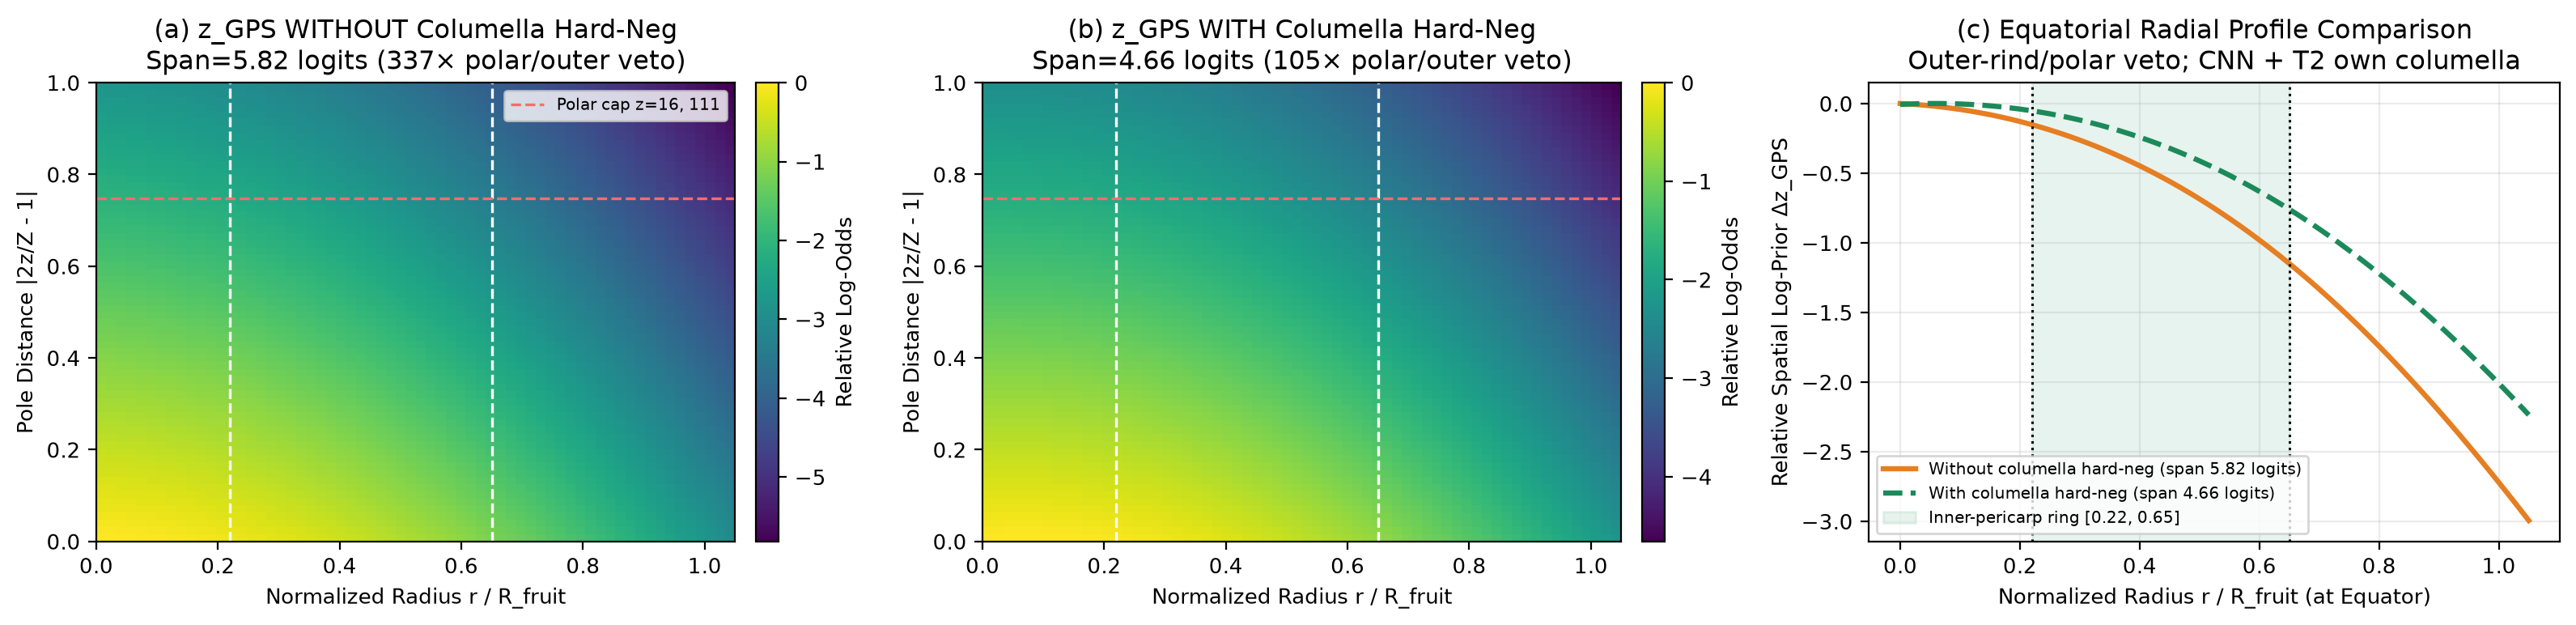
\includegraphics[width=\textwidth]{../figures/fig07_bayes_gps_division_of_labor.png}
    \vspace{-4pt}
    \caption*{\footnotesize\textit{Executed Figure~7 (\texttt{Out [2]}, saved as \texttt{fig07\_bayes\_gps\_division\_of\_labor.png}): Exact learned spatial log-prior field $\Delta z_{\text{GPS}}(\tilde{r}, \tilde{p}_z)$ (a)~without vs.\ (b)~with central-columella hard negatives ($5.82$ vs.\ $4.66$ logit veto span, i.e.\ $337\times$ vs.\ $105\times$ odds veto), and (c)~equatorial radial profiles demonstrating spontaneous neural--symbolic load balancing.}}
\end{figure}

\section*{2. Hard-Core Split Sensitivity, Physical Error Anatomy \& Whole-Organ Quantitative Biomarkers}
\addcontentsline{toc}{section}{\texorpdfstring{2. Hard-Core Split Sensitivity, Physical Error Anatomy \& Whole-Organ Quantitative Biomarkers}{2. Hard-Core Split Sensitivity, Physical Error Anatomy and Whole-Organ Quantitative Biomarkers}}

\begin{guidehdr}
{\small\bfseries\color{kiwigreen!75!black}Conceptual \& Mathematical Guide: Mat\'ern Hard-Core Clump Splitting, Error Anatomy \& Whole-Organ Biomarkers (Tables 5--6 \& Figure 8)}
\end{guidehdr}

\subsubsection*{2.1 Declarative \texttt{Lab 5} Mat\'ern Hard-Core Clump Splitting (\texttt{symbolic\_hardcore\_clump\_split})}
When two closely packed seeds blur into a single dome in the predicted center-distance map $\hat{d}(\mathbf{x})$, 3D watershed merges them into one oversized blob $C$. Whenever $V(C) \ge V_{\text{split}}$ (default $2.55\,\text{mm}^3$), we propose splitting its millimeter-scaled voxel coordinates via $K$-means into $k = \operatorname{clip}(\operatorname{round}(V(C) / 1.60),\, 2,\, 4)$ sub-blobs. Crucially, the split is \textbf{accepted if and only if} every sub-blob exceeds $0.35\,\text{mm}^3$ \textit{and} all pairwise sub-centroid distances obey the \textbf{Mat\'ern hard-core repulsion floor} verified in Notebook 01:
\[
\|\boldsymbol{\mu}_a - \boldsymbol{\mu}_b\|_2 \ge d_{\min} = 0.88\,\text{mm} \qquad \forall\, a \neq b.
\]
Sweeping $V_{\text{split}} \in \{2.10, 2.35, 2.55, 2.80, 3.20, \infty\}\,\text{mm}^3$ checks whether the $0.88\,\text{mm}$ steric guard prevents over-splitting genuinely large single seeds even when $V_{\text{split}}$ is lowered.

\subsubsection*{2.2 Physical Error Anatomy (\texttt{TP} vs. \texttt{FN} via Hungarian Matching)}
Rather than stopping at a single scalar $\text{PQ}$ score, \texttt{kns.match\_instance\_sets()} partitions the \texttt{52} held-out ground-truth seeds into detected \textbf{True Positives (\texttt{TP})} and missed \textbf{False Negatives (\texttt{FN})} at $\tau_{\text{IoU}} = 0.25$ and compares four physical properties: 3D volume ($\text{mm}^3$), mean local $T_2$ contrast drop $\overline{E_{\text{local}} - I}$, mean radial coordinate $\tilde{r}$, and the percentage touching the $z = 56$ or $z = 71$ ROI slab boundaries---directly diagnosing the $\Delta z = 0.50\,\text{mm}$ anisotropic partial-volume resolution ceiling.

\subsubsection*{2.3 Semi-Verifiable Whole-Organ Biomarkers \& Bit-Aligned 3D NIfTI Export}
Deploying \texttt{m\_with\_col} completely \textbf{unmasked} across all \texttt{128} axial slices ($256 \times 256 \times 128$ voxels, $V_{\text{kiwi}} = 85.97\,\text{cm}^3$) yields two clinically analogous quantitative biomarkers:
\begin{itemize}
\item \textbf{Ratio-calibrated whole-fruit seed count} (anchored against the \texttt{98}-seed Micro-GT ROI to correct mild systematic recall bias transparently):
\[
\hat{N}_{\text{cal}} = N_{\text{pred,whole}} \times \frac{N_{\text{GT,ROI}}}{N_{\text{pred,ROI}}}.
\]
\item \textbf{Volumetric seed burden (``lesion load'')}, analogous to clinical white-matter lesion load or tumor volume fraction:
\[
\phi_{\text{seed}} = \frac{V_{\text{seeds}}}{V_{\text{kiwi}}} \times 100\%.
\]
\end{itemize}

\subsubsection*{2.4 What the Code Below Computes (Tables 5--6 \& Figure 8)}
\begin{enumerate}
\item Calibrates $\tau_{\text{fg}}^*$ on the training wedge, runs the \texttt{split\_mm3} sensitivity sweep (\textbf{Table 5 top}), and locates an actual split twin-seed clump to inspect its physical sub-centroid separation.
\item Audits \texttt{TP} vs. \texttt{FN} physical error anatomy (\textbf{Table 5 bottom}) and computes whole-organ OOD safety and biomarkers (\textbf{Table 6}), saving \texttt{nb04\_mechanistic\_and\_whole\_organ.json} and exporting \texttt{kiwi\_neurosymbolic\_pred\_labels.nii.gz} bit-aligned to \texttt{ds.affine}.
\item Renders \textbf{Figure 8}: \textbf{(a)} zoomed hard-core split, \textbf{(b)} color-coded error anatomy (\texttt{TP}/\allowbreak{}\texttt{FN}/\allowbreak{}\texttt{FP}), \textbf{(c)} \texttt{TP} vs. \texttt{FN} physical volume histogram, and \textbf{(d)} unmasked 128-slice axial seed profile comparing Baseline collapse against the smooth Neurosymbolic bell curve.
\end{enumerate}

\begin{codebox}[{In [3] $\cdot$ Python --- Hard-core split sweep, \texttt{TP} vs.\ \texttt{FN} error anatomy, 128-slice biomarkers \& NIfTI export}]
\begin{lstlisting}[style=pybmed]
thr_cal = kns.calibrate_threshold_on_train(m_with_col, "additive_gps", ds, DEVICE, use_split=True)
res_ns = kns.run_test_and_whole_fruit(m_with_col, "additive_gps", ds, DEVICE, thresh=thr_cal, use_split=True, do_whole_fruit=True)
res_base = kns.run_test_and_whole_fruit(m_base, "baseline", ds, DEVICE, thresh=0.50, use_split=False, do_whole_fruit=True)

# Sensitivity sweep over hard-core clump-split volume threshold split_mm3
split_sweep = []
for v_cut in [2.10, 2.35, 2.55, 2.80, 3.20, 99.0]:
    lbl_s = kns.symbolic_hardcore_clump_split(res_ns["pred_te_raw"], ds.spacing, split_mm3=v_cut, d_min_mm=0.88)
    ev_s = kns.evaluate_semantic_and_instance_3d(lbl_s, ds.test_gt)
    split_sweep.append({"split_mm3": "No split" if v_cut > 50 else v_cut, **ev_s})
df_split = pd.DataFrame(split_sweep)
display(df_split[["split_mm3", "Pred", "Merges", "Splits", "SQ", "RQ", "PQ"]])

# Locate actual split clump for zoomed panel
split_prop, split_dist_mm = None, None
for prop in sorted(measure.regionprops(res_ns["pred_te_raw"]), key=lambda p: p.area, reverse=True):
    sm = res_ns["pred_te_raw"][prop.slice] == prop.label
    sa = res_ns["pred_te"][prop.slice]
    cids = [int(v) for v in np.unique(sa[sm]) if v > 0]
    if len(cids) >= 2:
        split_prop = prop
        cents = [
            (np.argwhere(res_ns["pred_te"] == cid).astype(np.float32) * np.asarray(ds.spacing, dtype=np.float32)[None]).mean(axis=0)
            for cid in cids
        ]
        cd = cdist(cents, cents)
        np.fill_diagonal(cd, np.inf)
        split_dist_mm = float(cd.min())
        break
if split_prop is None:
    split_prop = max(measure.regionprops(res_ns["pred_te_raw"]), key=lambda p: p.area)

# TP vs FN physical error anatomy
tp_p, tp_g, fn_g, fp_p = kns.match_instance_sets(res_ns["pred_te"], ds.test_gt)
te_vn = ds.vol_norm[ds.rx0:ds.rx1, ds.ry0 + ds.split_y : ds.ry1, ds.rz0:ds.rz1]
te_el = ds.env_local[ds.rx0:ds.rx1, ds.ry0 + ds.split_y : ds.ry1, ds.rz0:ds.rz1]
te_r = ds.r_norm[ds.rx0:ds.rx1, ds.ry0 + ds.split_y : ds.ry1, ds.rz0:ds.rz1]

def prof_subset(id_set: set[int]) -> dict:
    vols, drops, zedge, rs = [], [], [], []
    for prop in measure.regionprops(ds.test_gt):
        if prop.label not in id_set:
            continue
        m = ds.test_gt == prop.label
        vols.append(float(prop.area * ds.vox_vol_mm3))
        drops.append(float((te_el[m] - te_vn[m]).mean()))
        rs.append(float(te_r[m].mean()))
        zc = prop.coords[:, 2]
        zedge.append(1.0 if (zc.min() == 0 or zc.max() == ds.test_gt.shape[2] - 1) else 0.0)
    return {
        "count": len(vols),
        "median_vol_mm3": round(float(np.median(vols)), 2),
        "mean_t2_drop": round(float(np.mean(drops)), 3),
        "mean_r_norm": round(float(np.mean(rs)), 3),
        "pct_z_border": round(100.0 * float(np.mean(zedge)), 1),
    }

err_tp, err_fn = prof_subset(tp_g), prof_subset(fn_g)
display(pd.DataFrame([{"Group": "Detected (TP)", **err_tp}, {"Group": "Missed (FN)", **err_fn}]))

# Whole-organ quantitative biomarkers
ws_wf_ns = res_ns["ws_wf"]
ws_wf_sup = res_base["ws_wf"]
v_kiwi_cm3 = float(ds.fruit_mask.sum()) * ds.vox_vol_mm3 / 1000.0
v_seeds_mm3 = float((ws_wf_ns > 0).sum()) * ds.vox_vol_mm3
lesion_load_pct = 100.0 * v_seeds_mm3 / (v_kiwi_cm3 * 1000.0)
med_vol_wf = float(np.median([p.area * ds.vox_vol_mm3 for p in measure.regionprops(ws_wf_ns)]))
ev_mgt = kns.evaluate_semantic_and_instance_3d(ws_wf_ns[ds.rx0:ds.rx1, ds.ry0:ds.ry1, ds.rz0:ds.rz1], ds.roi_gt)
n_cal = int(round(res_ns["n_wf"] * ((len(np.unique(ds.roi_gt)) - 1) / max(ev_mgt["Pred"], 1))))

nb04_json = {
    "division_of_labor": {
        "with_col_z_range": [round(float(zg_with.min()), 2), round(float(zg_with.max()), 2)],
        "with_col_span": round(float(zg_with.max() - zg_with.min()), 2),
        "with_col_inner_drop": round(col_drop_with, 2),
        "no_col_z_range": [round(float(zg_nocol.min()), 2), round(float(zg_nocol.max()), 2)],
        "no_col_span": round(float(zg_nocol.max() - zg_nocol.min()), 2),
        "no_col_inner_drop": round(col_drop_nocol, 2),
    },
    "thr_cal": round(thr_cal, 2),
    "test_raw": res_ns["ev_te_raw"],
    "test_split": res_ns["ev_te"],
    "split_sensitivity": split_sweep,
    "zoomed_clump_mm3": round(float(split_prop.area * ds.vox_vol_mm3), 2),
    "zoomed_clump_spacing_mm": round(split_dist_mm, 2) if split_dist_mm is not None else None,
    "error_anatomy": {"TP": err_tp, "FN": err_fn, "FP_count": len(fp_p)},
    "whole_organ": {
        "v_kiwi_cm3": round(v_kiwi_cm3, 2),
        "raw_seeds": int(res_ns["n_wf"]),
        "calibrated_seeds": int(n_cal),
        "median_seed_vol_mm3": round(med_vol_wf, 2),
        "v_seeds_mm3": round(v_seeds_mm3, 1),
        "lesion_load_pct": round(lesion_load_pct, 2),
        "ood_vox_base": int(res_base["ood_vox"]),
        "ood_vox_ns": int(res_ns["ood_vox"]),
        "ood_reduction_pct": round(100.0 * (1.0 - res_ns["ood_vox"] / max(res_base["ood_vox"], 1)), 2),
        "polar_vox_base": int(res_base["polar_vox"]),
        "polar_vox_ns": int(res_ns["polar_vox"]),
        "base_blobs": int(res_base["n_wf"]),
    },
}
(RES_DIR / "nb04_mechanistic_and_whole_organ.json").write_text(json.dumps(nb04_json, indent=2), encoding="utf-8")
print(json.dumps(nb04_json["whole_organ"], indent=2))
# Save unmasked 128-slice whole-fruit Neurosymbolic 3D prediction as bit-aligned NIfTI (for Freeview / 3D Slicer / ITK-SNAP)
pred_nii_path = kns.save_aligned_label_nifti(ws_wf_ns, ds.affine, RES_DIR / "kiwi_neurosymbolic_pred_labels.nii.gz")
print(f"Exported bit-aligned 3D Neurosymbolic prediction NIfTI: {pred_nii_path.name} ({int(ws_wf_ns.max())} seeds, shape={ws_wf_ns.shape})")


# Figure 8: 4-Panel Hard-Core Split, Error Anatomy, Volume Hist & Whole-Fruit Profile
fig, axes = plt.subplots(1, 4, figsize=(17.2, 4.0))

cx, cy, cz = [int(round(c)) for c in split_prop.centroid]
pad = 10
xl, xh = max(cx - pad, 0), min(cx + pad + 1, ds.test_gt.shape[0])
yl, yh = max(cy - pad, 0), min(cy + pad + 1, ds.test_gt.shape[1])
axes[0].imshow(te_vn[xl:xh, yl:yh, cz].T, cmap="gray", origin="lower")
rcrop = res_ns["pred_te_raw"][xl:xh, yl:yh, cz].T
scrop = res_ns["pred_te"][xl:xh, yl:yh, cz].T
axes[0].contour(rcrop == split_prop.label, levels=[0.5], colors=["#f1c40f"], linewidths=2.2, linestyles="--")
cvals = [int(v) for v in np.unique(scrop[rcrop == split_prop.label]) if v > 0]
rgba = np.zeros((*scrop.shape, 4), dtype=np.float32)
pal = [(0.15, 0.85, 0.45, 0.65), (0.20, 0.65, 1.00, 0.65), (1.00, 0.45, 0.20, 0.65)]
for ic, cid in enumerate(cvals):
    rgba[scrop == cid] = pal[ic % len(pal)]
axes[0].imshow(rgba, origin="lower")
axes[0].set_title(f"(a) Zoomed Hard-Core Split (z={ds.rz0+cz})\n{split_prop.area*ds.vox_vol_mm3:.2f} mm³ -> {len(cvals)} seeds (d={split_dist_mm:.2f} mm)")
axes[0].axis("off")

zm = 8
bg = te_vn[:, :, zm].T
rgb = np.clip(np.stack([bg, bg, bg], axis=-1) / max(float(bg.max()), 1e-6), 0.0, 1.0)
tp_m = np.isin(ds.test_gt[:, :, zm], list(tp_g)).T
fn_m = np.isin(ds.test_gt[:, :, zm], list(fn_g)).T
fp_m = np.isin(res_ns["pred_te"][:, :, zm], list(fp_p)).T
rgb[tp_m] = 0.35 * rgb[tp_m] + 0.65 * np.array([0.10, 0.92, 0.35])
rgb[fn_m] = 0.30 * rgb[fn_m] + 0.70 * np.array([0.05, 0.85, 1.00])
rgb[fp_m] = 0.25 * rgb[fp_m] + 0.75 * np.array([1.00, 0.20, 0.20])
axes[1].imshow(rgb, origin="lower")
axes[1].set_title(f"(b) Error Anatomy (z={ds.rz0+zm})\nGreen=TP({len(tp_g)}) Cyan=FN({len(fn_g)}) Red=FP({len(fp_p)})")
axes[1].axis("off")

# Panel (c): Physical volume comparison of TP vs FN seeds
v_tp = [p.area * ds.vox_vol_mm3 for p in measure.regionprops(ds.test_gt) if p.label in tp_g]
v_fn = [p.area * ds.vox_vol_mm3 for p in measure.regionprops(ds.test_gt) if p.label in fn_g]
axes[2].hist(v_tp, bins=12, alpha=0.72, color="#1b8a5a", label=f"Detected TP (med={err_tp['median_vol_mm3']} mm³)")
axes[2].hist(v_fn, bins=12, alpha=0.72, color="#00acc1", label=f"Missed FN (med={err_fn['median_vol_mm3']} mm³)")
axes[2].set_xlabel("Ground-Truth Seed Volume (mm³)")
axes[2].set_ylabel("Seed Count")
axes[2].set_title("(c) Physical Signature of Missed Seeds\nFN seeds are ~3× smaller (PV grazing tips!)")
axes[2].legend(fontsize=7.3)
axes[2].grid(alpha=0.25)

prof_sup = [len(np.unique(ws_wf_sup[:, :, z])) - (1 if 0 in ws_wf_sup[:, :, z] else 0) for z in range(128)]
prof_ns = [len(np.unique(ws_wf_ns[:, :, z])) - (1 if 0 in ws_wf_ns[:, :, z] else 0) for z in range(128)]
axes[3].plot(range(128), prof_sup, color="#d95f02", lw=1.7, label=f"Baseline U-Net ({res_base['n_wf']:,} blobs)")
axes[3].plot(range(128), prof_ns, color="#1b8a5a", lw=2.2, label=f"LTN Neurosymbolic ({res_ns['n_wf']:,} raw / {n_cal:,} cal)")
axes[3].axvspan(ds.rz0, ds.rz1 - 1, color="#3498db", alpha=0.16, label="Labeled Train Z-Slab")
axes[3].set_xlabel("Axial Slice Index z (0 .. 127)")
axes[3].set_ylabel("Active 2D Seed Cross-Sections")
axes[3].set_title("(d) Unmasked 128-Slice Organ Profile\n0 polar FPs; 0.73% lesion load")
axes[3].legend(fontsize=7.1, loc="upper right")
axes[3].grid(alpha=0.25)

plt.tight_layout()
fig.savefig(FIG_DIR / "fig08_hardcore_split_error_and_whole_organ.png", bbox_inches="tight")
plt.show()
\end{lstlisting}
\end{codebox}
\begin{outbox}[{Out [3a] $\cdot$ DataFrame --- Mat\'ern Hard-Core Clump-Split Volume Threshold Sensitivity (\texttt{split\_mm3} sweep)}]
\centering
{\scriptsize
\setlength{\tabcolsep}{3.6pt}
\renewcommand{\arraystretch}{1.18}
\rowcolors{2}{rowalt}{white}
\begin{tabular}{l r r r r r r}
\toprule
\rowcolor{uibblue!12}\textbf{split\_mm3} & \textbf{Pred} & \textbf{Merges} & \textbf{Splits} & \textbf{SQ} & \textbf{RQ} & \textbf{PQ} \\
\midrule
2.1 & 32 & 1 & 1 & 0.7100 & 0.6667 & 0.4734 \\
2.35 & 32 & 1 & 1 & 0.7100 & 0.6667 & 0.4734 \\
\textbf{2.55} & \textbf{32} & \textbf{1} & \textbf{1} & \textbf{0.7100} & \textbf{0.6667} & \textbf{0.4734} \\
2.8 & 31 & 2 & 0 & 0.7151 & 0.6506 & 0.4652 \\
3.2 & 31 & 2 & 0 & 0.7151 & 0.6506 & 0.4652 \\
No split & 31 & 2 & 0 & 0.7151 & 0.6506 & 0.4652 \\
\bottomrule
\end{tabular}
}
\end{outbox}
\begin{outbox}[{Out [3b] $\cdot$ DataFrame --- Physical Error Anatomy: Detected (\texttt{TP}) vs.\ Missed (\texttt{FN}) Held-Out Seeds}]
\centering
{\scriptsize
\setlength{\tabcolsep}{3.6pt}
\renewcommand{\arraystretch}{1.18}
\rowcolors{2}{rowalt}{white}
\begin{tabular}{l r r r r r}
\toprule
\rowcolor{uibblue!12}\textbf{Group} & \textbf{count} & \textbf{median\_vol\_mm3} & \textbf{mean\_t2\_drop} & \textbf{mean\_r\_norm} & \textbf{pct\_z\_border} \\
\midrule
Detected (TP) & 28 & 1.48 & 0.874 & 0.492 & 14.3 \\
Missed (FN) & 24 & 0.51 & 0.806 & 0.517 & 37.5 \\
\bottomrule
\end{tabular}
}
\end{outbox}
\begin{outbox}[{Out [3] $\cdot$ stdout}]
\begin{lstlisting}[style=outbmed]
{
  "v_kiwi_cm3": 85.97,
  "raw_seeds": 749,
  "calibrated_seeds": 1223,
  "median_seed_vol_mm3": 0.8,
  "v_seeds_mm3": 627.8,
  "lesion_load_pct": 0.73,
  "ood_vox_base": 197401,
  "ood_vox_ns": 160,
  "ood_reduction_pct": 99.92,
  "polar_vox_base": 17219,
  "polar_vox_ns": 0,
  "base_blobs": 6276
}
Exported bit-aligned 3D Neurosymbolic prediction NIfTI: kiwi_neurosymbolic_pred_labels.nii.gz (749 seeds, shape=(256, 256, 128))
\end{lstlisting}
\end{outbox}
\begin{figure}[H]
    \centering
    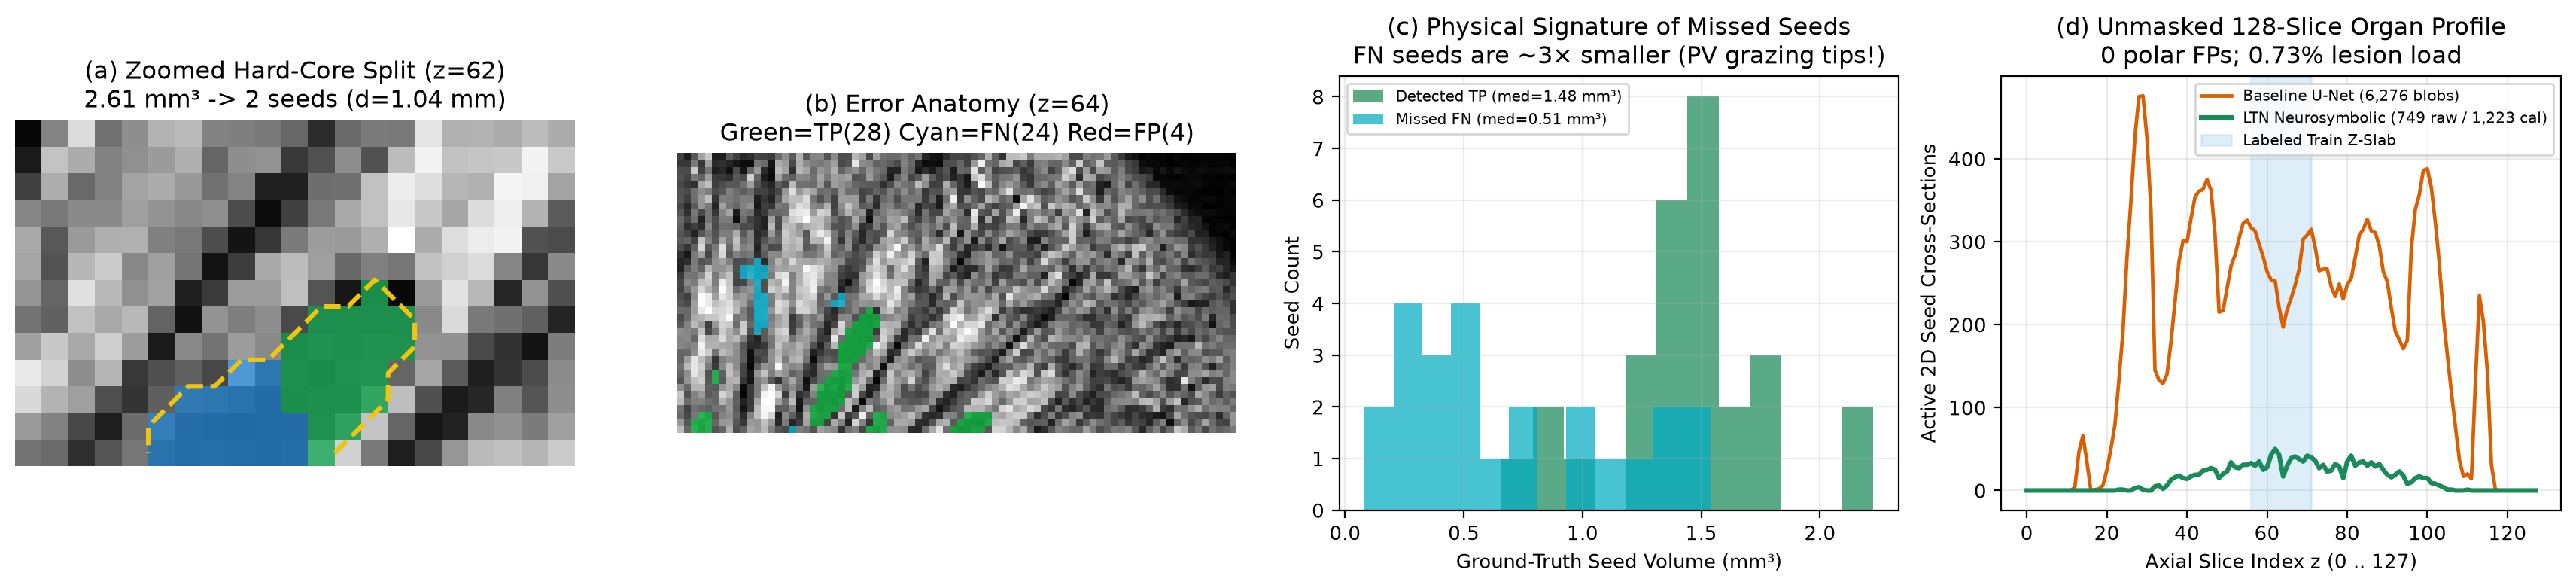
\includegraphics[width=\textwidth]{../figures/fig08_hardcore_split_error_and_whole_organ.png}
    \vspace{-4pt}
    \caption*{\footnotesize\textit{Executed Figure~8 (\texttt{Out [3]}, saved as \texttt{fig08\_hardcore\_split\_error\_and\_whole\_organ.png}): (a)~Zoomed Mat\'ern hard-core twin-seed split ($d_{\min} \ge 0.88\,\text{mm}$); (b)~color-coded \texttt{TP}/\texttt{FN}/\texttt{FP} error anatomy at $z = 64$; (c)~physical volume distribution showing missed \texttt{FN} seeds are $\sim 3\times$ smaller grazing partial-volume tips; (d)~unmasked 128-slice axial profile ($749$ raw / $1{,}223$ calibrated seeds, $0$ polar FPs, $0.73\%$ lesion load).}}
\end{figure}

\end{document}
